% TO-DO:
% * 立法机制
% * 

\documentclass[10pt]{beamer}

\usepackage[CJKspace]{xeCJK}
% \setCJKmainfont[BoldFont=Alibaba PuHuiTi Bold,ItalicFont=AR PL KaitiM GB]{Alibaba PuHuiTi Light}
\setCJKmainfont[ItalicFont=AR PL KaitiM GB]{Alibaba PuHuiTi}
\setmainfont[ItalicFont=Latin Modern Roman Slanted]{Alibaba Sans:style=Light}

%\usepackage{newtxtext,newtxmath}	% use Times Roman font
\usepackage{newtxtext}
\renewcommand{\familydefault}{\sfdefault}
%\usefonttheme{serif}
\usefonttheme{professionalfonts}
%\setbeamertemplate{theorems}[numbered]
\setbeamertemplate{caption}{\insertcaption} 	% no `Figure' prefix before caption

\mode<presentation> {

\usetheme{default}
%\usetheme{AnnArbor}
%\usetheme{Antibes}
%\usetheme{Bergen}
%\usetheme{Berkeley}
%\usetheme{Berlin}
%\usetheme{Boadilla}
%\usetheme{CambridgeUS}
%\usetheme{Copenhagen}
%\usetheme{Darmstadt}
%\usetheme{Dresden}
%\usetheme{Frankfurt}
%\usetheme{Goettingen}
%\usetheme{Hannover}
%\usetheme{Ilmenau}
%\usetheme{JuanLesPins}
%\usetheme{Luebeck}
%\usetheme{Madrid}
%\usetheme{Malmoe}
%\usetheme{Marburg}
%\usetheme{Montpellier}
%\usetheme{PaloAlto}
%\usetheme{Pittsburgh}
%\usetheme{Rochester}
%\usetheme{Singapore}
%\usetheme{Szeged}
%\usetheme{Warsaw}

%\usecolortheme{albatross}
%\usecolortheme{beaver}
%\usecolortheme{beetle}
%\usecolortheme{crane}
\usecolortheme{dolphin}
%\usecolortheme{dove}
%\usecolortheme{fly}
%\usecolortheme{lily}
%\usecolortheme{orchid}
%\usecolortheme{rose}
%\usecolortheme{seagull}
%\usecolortheme{seahorse}
%\usecolortheme{whale}
%\usecolortheme{wolverine}

%\setbeamertemplate{footline} % To remove the footer line in all slides uncomment this line
\setbeamertemplate{footline}[page number] % To replace the footer line in all slides with a simple slide count uncomment this line
\setbeamertemplate{navigation symbols}{} % To remove the navigation symbols from the bottom of all slides uncomment this line
}

\setbeamertemplate{headline}{}
% \setbeamersize{text margin left=1mm,text margin right=4mm} 
%\settowidth{\leftmargini}{\usebeamertemplate{itemize item}}
%\addtolength{\leftmargini}{\labelsep}

% *************** BIBLIOGRAPHY STUFF ******************
% \usepackage[backend=biber,style=numeric]{biblatex}
% \bibliography{../AGI-book}
% \bibliography{../Economics}
% \renewcommand*{\bibfont}{\footnotesize}
% \setbeamertemplate{bibliography item}[text]

\usepackage{graphicx} % Allows including images
\usepackage{tikz-cd}
% \usepackage{ulem}
\usepackage[export]{adjustbox}% http://ctan.org/pkg/adjustbox
\usepackage{verbatim} % comments
% \usepackage{tikz-cd}  % commutative diagrams
% \newcommand{\tikzmark}[1]{\tikz[overlay,remember picture] \node (#1) {};}
% \usepackage{booktabs} % Allows the use of \toprule, \midrule and \bottomrule in tables
% \usepackage{amssymb}  % \leftrightharpoons
\usepackage{newtxtext,newtxmath}	% Times New Roman font
\usepackage{pict2e}		% pciture drawing polygon

\newcommand{\emp}[1]{{\color{blue}\textbf{#1}}}
\newcommand{\vect}[1]{\boldsymbol{#1}}
\newcommand{\tab}{\hspace*{1cm}}
\newcommand*\confoundFace{$\vcenter{\hbox{\includegraphics[scale=0.2]{../confounded-face.jpg}}}$}
\newcommand{\smiley}{$\vcenter{\hbox{\includegraphics[scale=0.05]{../smiling-face.png}}}$}

\makeatletter
\renewcommand{\boxed}[1]{\fbox{\m@th$\displaystyle\scalebox{0.9}{#1}$} \,}
\makeatother

\def\Put(#1,#2)#3{\leavevmode\makebox(0,0){\put(#1,#2){#3}}}

%----------------------------------------------------------------------------------------
%	TITLE PAGE
%----------------------------------------------------------------------------------------

\title[Genifer biz plan]{Genifer biz plan}
\author{HK.neutrality@gmail.com}
%\author{\cc{YKY 甄景贤}{YKY}} % Your name
%\institute[] % Your institution as it will appear on the bottom of every slide, may be shorthand to save space
%{
%Independent researcher, Hong Kong \\ % Your institution for the title page
%\medskip
%\textit{generic.intelligence@gmail.com} % Your email address
%}
\date{\today} % Date, can be changed to a custom date

\begin{document}

\usebackgroundtemplate{%
	\begin{picture}(600,220)
	\put(35,55){
\includegraphics[scale=1]{Genifer-square-logo.png}}
	\definecolor{graygray}{rgb}{.867,0.867,0.867}
	{\color{graygray}\polygon*(-20,-80)(-20,-5)(400,85)(400,-80)}
	\Put(240,-145){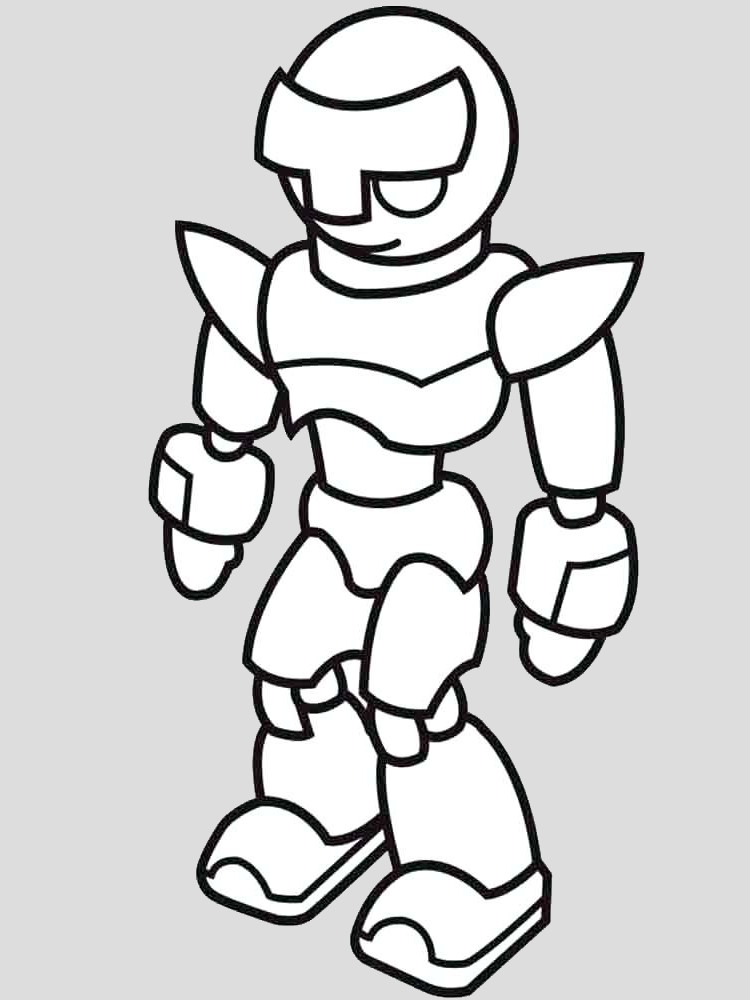
\includegraphics[scale=0.08]{robot1.jpg}}
	\end{picture}
}
% \addtocounter{page}{-1}
\begin{frame}[plain,noframenumbering]
% \titlepage
\end{frame}

\usebackgroundtemplate{
	\begin{picture}(600,220)
	\definecolor{graygray}{rgb}{.867,0.867,0.867}	{\color{graygray}\polygon*(-20,-80)(-20,-5)(400,85)(400,-80)}
	\end{picture}
}

%\addtocounter{page}{-1}
%\begin{frame}[noframenumbering]
%\frametitle{Table of contents}
%\listofframes
%\vspace*{0.5cm}
%多谢 各界支持 \smiley
%\end{frame}

%----------------------------------------------------------------------------------------
%	PRESENTATION SLIDES
%----------------------------------------------------------------------------------------

%------------------------------------------------

\begin{frame}
% \frametitle{Business strategy}
%\fontsize{7pt}{7.2}\selectfont
\vspace*{2em}
{\color{blue} \Huge \textbf{Business strategy}}
\begin{itemize}
	\item 这是一个 \emp{全球化} 的项目,not based in any particular country, \\
			所有人可以参与,促进国际间合作
	
	\item 我们组织的宗旨,是消除任何 种族/国籍的歧视
	
	\item 奖励机制 纯粹由对项目的贡献而定,可以用未来的人工智能 \emp{追溯}
\end{itemize}
\end{frame}

\begin{frame}
\vspace*{2em}
{\color{blue} \Huge \textbf{关於我的 AI 理论}}
\begin{itemize}
	\item architecture is based on \emp{reinforcement learning} \\
			(这是很「标准」的架构,例如捉围棋的 Alpha-Go)
	
	\item 另一部分是 结合 \emp{深度学习} 和 \emp{逻辑} \\
			(這部分比較複雜,特別是數理邏輯的最新理論) 
\end{itemize}
\vspace*{1em}
{\small 业馀 看书学习 Tensorflow 的人}
\end{frame}

\begin{frame}
\vspace*{2em}
{\color{blue} \Large \textbf{What remains to be done}}

\vspace{0.5em}
\hspace*{5em}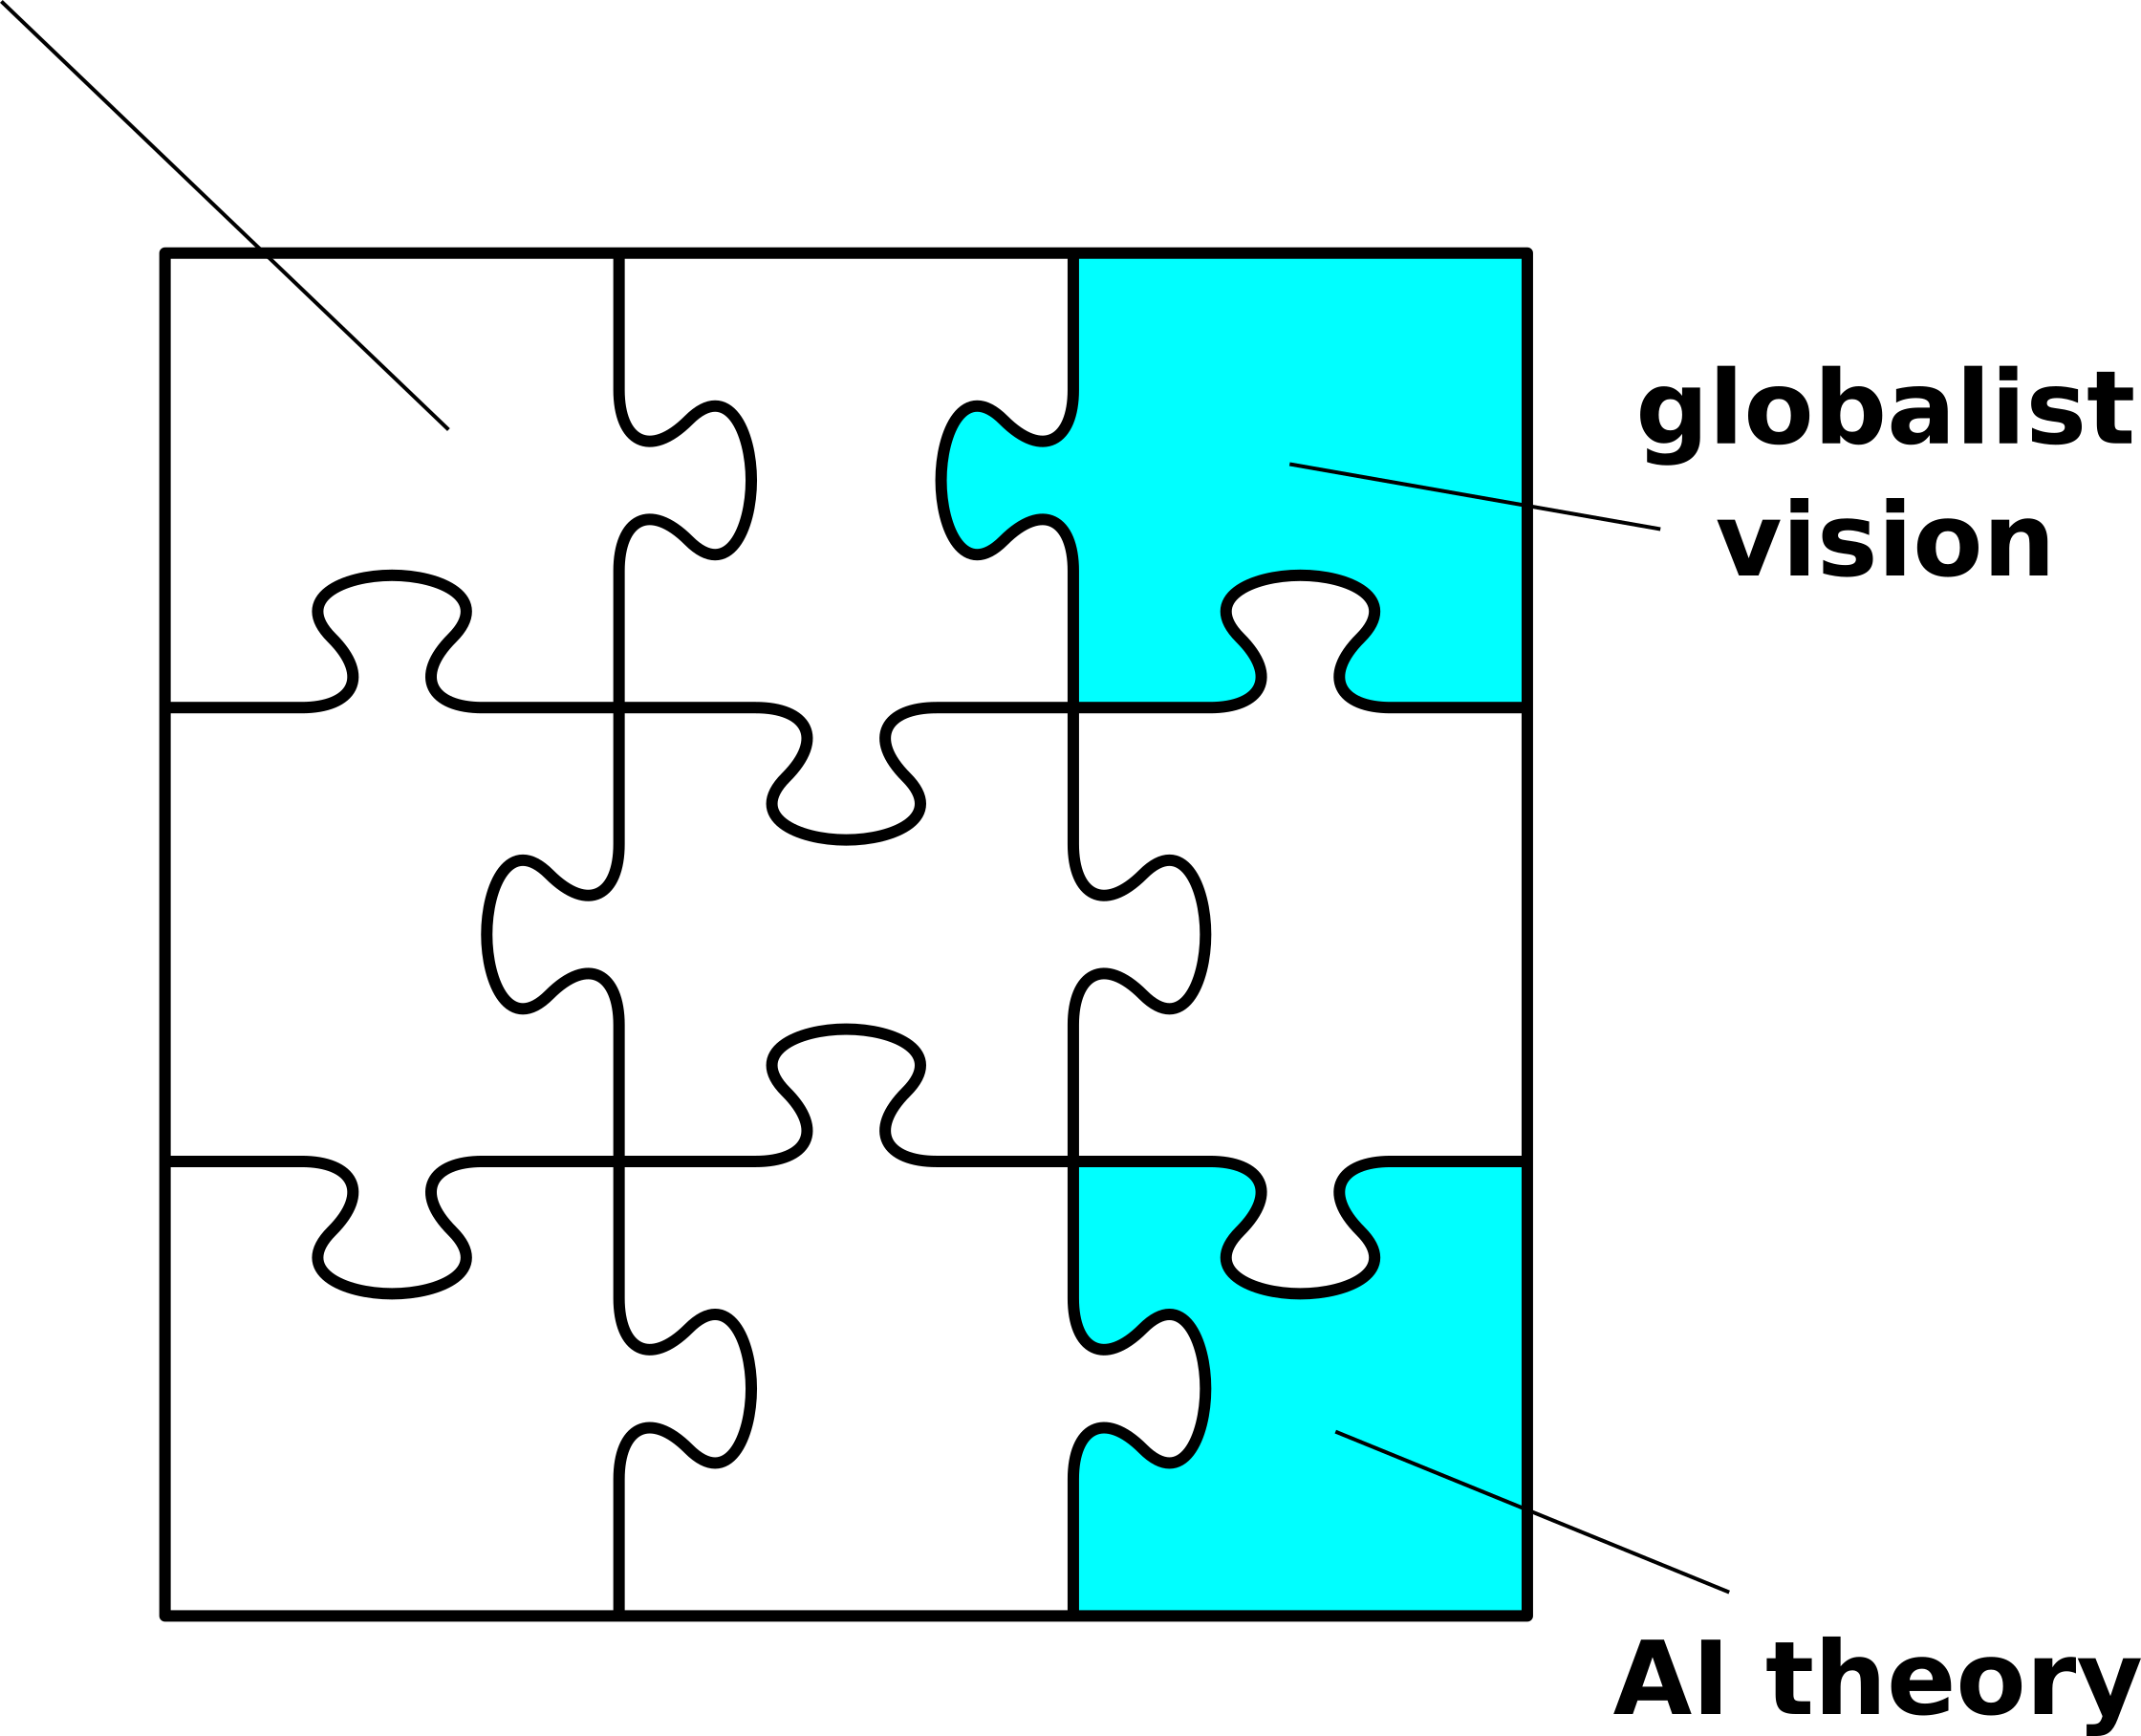
\includegraphics[scale=0.4]{jigsaw-puzzle.png}
\end{frame}

\end{document} 